\documentclass{article}

%table customization, stack overflow 
\usepackage{array}
\newcolumntype{L}[1]{>{\raggedright\let\newline\\
\arraybackslash\hspace{0pt}}m{#1}}

%figure flaots from http://www.tex.ac.uk/FAQ-figurehere.HTML
\usepackage{float}
\usepackage{ltablex}
\usepackage{tabularx}
\usepackage{enumitem}
\usepackage{graphicx}
\usepackage{booktabs}
\usepackage{url}
\usepackage{hyperref}
\usepackage{fancyhdr}
\pagestyle{fancy}
\begin{document}
\pagenumbering{gobble}
\lhead{Team 6\\ JSTanks\\}
\newpage
\title{JSTanks - Design Document}
\date{December 8, 2016}
\author{Jiahao Li\\LI577\\001416646\and Pavithran Pathmarajah\\PATHMAP\\
001410729 \and Viren Patel\\PATELVH3\\001419057}

\maketitle

\newpage
\pagenumbering{arabic}
\tableofcontents

\newpage
\section{Revision History}
\begin{table}[H]
\caption{Revision History}
	\begin{tabularx}{\textwidth}{cXcc}
		\toprule
		Date & Developer & Change&Revision\\
		\midrule
		November 6&Jiahao Li &Initial Draft&0 \\
		November 6&Pavithran Pathmarajah &Initial Draft&0\\
		November 6&Viren Patel  &Initial Draft&0\\
		December 7&Viren Patel &Final Draft&1\\
	\end{tabularx}
\end{table}

\section{Introduction}
Module Decomposition is a good practice when it comes to developing applications involving many different data structures. Following this can benefit the program in many ways including the implementation process, maintenance, testing, and understanding of the program to new entities.\\ \\
This document is a Module Guide for JSTanks. JSTanks has followed the process the Module Decomposition greatly and can be seen in this doument.This document goes in to detail to show how the things mentioned in the Software Requirements Specifications document are accomplished in the program. It shows how the functions of the program are executed as the modules interact with eachother and tracing each function to its corresponding module(s). \\ \\
This document has been divided into the following sections: Anticipated and Unlikely Changes of the software requirements, Module Hierarchy, Connection between Requirements and Design, Module Decomposition, Traceability Matrix, and Use Hierarchy between Modules.

\section{Anticipated and Unlikely Changes}
This sections contains possible changes to the project which may occur. The changes are placed into two categories anticipated and unlikely, depending on how likely a change is to occur.

\subsection{Anticipated Changes}
Anticipated changes are sources within modules which may be modified throughs-out the products life time. The changes will be made to specific modules in such a way that it will not affect how modules interact, or respond, but how they work.
\subsubsection*{AC1}
Each tile pre-render's it's own image when it is created. Will be changed such that shared images are pre-rendered on startup
\subsubsection*{AC2}
Currently a single thread runs procedurally. Updated game will have a sole update and render thread in the background. Preventing browser lock up.
\subsubsection*{AC3}
Level and map specifications may be moved to an external text or Html file to be parsed by the game dynamically. Allowing for the addition of new maps without having to hardcode scripts.
\subsubsection*{AC4}
Artificial Intelligence of bots, to be replaced with an algorithm to try and attack the player tank and the home-base depending on what is closer. 
\subsubsection*{AC5}
The strength of projectiles to go down depending on number of grid spots away from the tank they have travelled.
\subsubsection*{AC6}
Only re-rendering changed entities instead of the current system where  all entities are re-rendered each frame.

\subsection{Unlikely Changes}
Unlikely changes are the changes that will most likely not occur, for the affects of these changes would require many modifications to many modules for it would have an effect on how modules interact and respond.
\subsubsection*{UC1}
The data that tile-entities store and provide will remain at a minimum of health information and graphics renders.
\subsubsection*{UC2}
The game will continue to be purely, HTML, CSS, an JavaScript such that it modules will not have to be ported to another language or ecosystem
\subsubsection*{UC3} 
All interfacing between entities and the user will continue to propagate through the gameBoard class.
\subsubsection*{UC4}
  Game graphics will not be changed from a three level render stack to, a two level stack. Since it would require changes across all modules.

\section{Module Hierarchy} \label{sec:Module_Hierarchy}
This section provides a simple overview of the module design. The modules are hierarchically labelled M1 through M13 below and are decomposed in the table below that. 
\\
Hierarchy. These are the modules which will be implemented.
\\ \\M1: Game Module
\\M2: GameBoard Module
\\M3: Projectile Queue Module
\\M4: Create Game Module
\\M5: Player Module
\\M6: Bot Module
\\M7: Tank Module
\\M8: Empty Tile Module
\\M9: Projectile Module
\\M10: Home-Base Module
\\M11: Wall-Module
\\M12: Steel-Wall Module
\\M13: Overlay Module
\\M14: JSTanks Web Module
\\M15: JSTanks Style Module

%space used to move table to next page
 % \caption{Module Hierarchy}
\begin{tabularx}{\textwidth}{l X}

	Level 1 & Level 2\\
	\midrule
	Game Module & - Set graphics area\\ \\
	 & - Create graphics context\\ \\
	 & - start main game loop\\ \\
	 & - interface between key presses, Overlay menu and GameBoard\\ \\
	 & - GameBoard Module\\ \\
	 & - Overlay menu\\
	 \midrule
	 GameBoard Module & - Interface between user and game\\ \\
	 & - update board graphics\\ \\
	 & - update projectiles\\ \\
	 & - move entities on request\\ \\
	 & - Create Game Module \\ \\
	 & - Projectile  QueueModule \\ \\
	 & - Player Module\\ \\
	 & - Bot Module\\ \\
	 & - Wall Module\\ \\
	 & - Steel-Wall Module\\ \\
	 & - Home-Base Module\\ \\
	 & - Empty Tile Module\\
	  \midrule
	 Projectile  Queue Module & - Array of Projectiles \\ \\
	 & - draw projectiles on board\\ \\
	 & - Projectile Module\\
	  \midrule
	 Create Game Module & - Place tiles on board \\ \\
	 & - Player Module\\ \\
	 & - Bot Module\\ \\
	 & - Wall Module\\ \\
	 & - Steel-Wall Module\\ \\
	 & - Home-Base Module\\
	  \midrule
	 Player Module & - Keyboard interfacing with tank\\ \\
	 & - Tank Module\\
	   \midrule
	 Bot Module & - Artificial Intelligence interfacing  with tank\\ \\
	 & - Tank Module\\
	 \midrule
	 Tank Module & - tank movement \\ \\
	 & - fire projectiles\\ \\
	 & - tracks tank health\\
	   \midrule
	 Empty Tile Module & - No strength factor \\ \\
	  & - Can be moved to\\ \\
	  & - replaces destroyed entities\\
	    \midrule
	 Projectile Module & - Damage tile entities \\ \\
	 & - identify tile hit\\
	  \midrule
	 Home-Base Module & - Player's home base will trigger end game on destroy \\ \\
	 & - tracks base health\\
	 \midrule 
	 Wall Module & - A weak wall, that can be destroyed \\ \\
	 & - tracks wall health\\
	 \midrule
	 Steel-Wall Module & - A stronger wall, that can take more damage \\ \\
	 & - tracks steel-wall health\\
	  \midrule
	 Overlay Module & - Pauses game loop \\ \\
	 & - overlay's pause menu\\
	\midrule
	JSTanks Web Module & -Displays the whole game on the website\\ \\
	\midrule
	JSTanks Style Module & -Styles the game's webpage\\ \\

\end{tabularx}

\section{Connection between Requirements and Design}
The requirements included in the Software Requirements Specifications document are implemented into the modules listed in the "Module Hierarchy" \ref{sec:Module_Hierarchy} section of this document.
The corresponding modules of all function and non-functional requirements can be found in Table \ref{tab:Traceability}  .


\section{Module Decomposition}
Modules are decomposed according to the principles of "information hiding" proposed by Parnas ed el (1984). We have made the design decision to not implement traditional information hiding, such that the project may be used by others whom are starting out in game design or programming, whom will be able to easily decipher our project and build their own web based game. By hiding how our key modules function internally, these new-comers will not be able to fully understand how to develop a basic HTML, CSS, JavaScript game; for this reason JSTanks has opted out from information hiding. All module decomposition can be found in the Module Interface Specification. 

\section{Traceability Matrix}
\begin{tabularx}{\textwidth}{l X}
        \toprule
        Requirement & Module(s) \\
        \midrule
        \multicolumn{2}{c}{Functional Requirements} \\
        \midrule \\
        FR1 & JSTanks Web \\
        FR2 & JSTanks Web\\
        FR3 & JSTanks Web, JSTanks Style, Game, Game Board, Home-Base, Wall, Steel-Wall, Create Game, Tank, Bot, Overlay \\
        FR4 & Overlay.\\
        FR5 & Overlay\\
        FR6 & Overlay \\
        FR7 & Overlay\\
        FR8 & Overlay\\
        FR9 & Overlay \\
        FR10 & Overlay \\
        FR11 & Overlay \\
        FR12 & Overlay\\
        FR13 & Bot, Projectile Queue, Tank \\
        FR14 & Bot\\
        FR15 & Bot\\
        FR16 & Overlay\\
        FR17 & Player, Tank\\
        FR18 & Projectile Queue\\
        FR19 & Projectile Queue, Tank, Bot\\
        FR20 & Game Board, Home-Base, Wall, Steel-wall, Projectile Queue\\
        FR21 & Game Board, Home-Base, Wall, Steel-wall, Projectile Queue\\
        FR22 & Game Board, Home-Base, Wall, Steel-wall, Projectile Queue\\
        FR23 & Projectile Queue, Tank, Player \\
        FR24 & Overlay \\
        FR25 & Overlay \\ \\
        \midrule
        \multicolumn{2}{c}{Non-functional Requirements} \\ 
        \midrule \\
        NF1.1 & JSTanks Web, JSTanks Style, Game, Game Board, Home-Base,  Wall, Steel-Wall, Create Game, Tank, Bot\\
        NF1.2 & JSTanks Web, JSTanks Style, Game, Game Board, Tank,  Bot, Overlay \\
        NF2.1 & Tank, Player, Projectile \\
        NF2.2 & -- \\
        NF2.3 & JSTanks Web\\
        NF2.4& Overlay \\
        NF2.5 & -- \\
        NF3 & -- \\
        NF4 &JSTanks Web, JSTanks Style \\
        NF5 & Game, Game Board, Tank, Player, Bot, Overlay, Home-Base, Wall, Steel-Wall, Create Game, Projectile Queue \\
        NF6 & -- \\
        NF7 & Overlay\\
        NF8 & -- \\ \\
	\midrule
        \multicolumn{2}{c}{Anticipated Changes} \\
        \midrule \\
	AC1&Game Board, Game\\
	AC2&Game, JSTanks Web\\
	AC3&Create Game, Game Board\\
	AC4&Bot\\
	AC5&Projectile\\
	AC6&Game Board, Game\\
        \bottomrule \\
        \caption{Trace Between Requirements and Modules}
        % Colour for the rulings in tables:
        \makeatletter
           \def\rulecolor#1#{\CT@arc{#1}}
           \def\CT@arc#1#2{%
           \ifdim\baselineskip=\z@\noalign\fi
           {\gdef\CT@arc@{\color#1{#2}}}}
           \let\CT@arc@\relax
          \rulecolor{black!50}
        \makeatother
        \label{tab:Traceability}
\end{tabularx}

\section{Use Relations}
\begin{figure}[H]
	\centering
	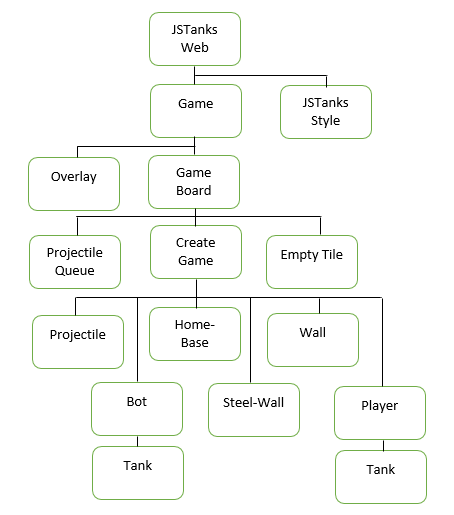
\includegraphics[width=\textwidth]{Uses_Hierarchy.png}
	\caption{Uses Hierarchy}
\end{figure}
\begin{table}[!h]
\begin{tabular}{lll}
Module && Use Relation \\ 
\hline \\
JSTanks Web&uses&JSTanks Style, Game\\ \\
JSTanks Style&uses&--\\ \\
Game&uses&Game Board, Overlay\\ \\
Game Board&uses&Projectile Queue, Create Game, Player, Bot, Empty Tile,\\
&& Home-Base, Wall, Steel-Wall	 \\ \\
Projectile Queue&uses&Projectile\\ \\
Create Game&uses&Player, Bot, Empty-Tile, Home-Base, Wall, Steel-Wall\\ \\
Player&uses&Tank\\ \\
Bot&uses&Tank\\ \\
Tank&uses&--\\ \\
Empty Tile&uses&--\\ \\
Projectile&uses&--\\ \\
Home-Base&uses&--\\ \\
Wall&uses&--\\ \\
Steel-Wall&uses&--\\ \\
Overlay&uses&--\\ \\
\hline
\end{tabular}
\caption {Uses Relationship between Modules}
\end{table}

\newpage
% Revision History, Module Hierarchy, Trace between Requirements and Modules, Trace between Anticipated Changes and Modules
\listoftables
% Use hierarchy among modules
\listoffigures

\end{document}